\section{The Virtual Machine}
\label{virtual_machine}

We have developed a compiler that compiles LM programs to byte-code
and a multithreaded virtual machine (VM) using POSIX threads
that runs the byte-code.

%%%%%%%%%%%%%%%%%%%%%%%%%%%%%%%%%%%%%%%%%%%%%%%%%%%%%%%%%%%%%%%%%%%%%%

\subsection{Threads}

A key goal of our design is to keep the threads as busy as possible
and to reduce inter-thread communication. When the VM starts, it reads
the byte-code file and starts all threads. Initially, the VM will
partition the application graph of $N$ nodes into $T$ subgraphs (the
number of threads) and then each thread will work on their own
subgraph. Reduction of communication between nodes in different threads
is achieved by first ordering the node addresses present in the code in such a way that
connected nodes are clustered together and then partitioning them to
threads. During compilation, we take note of predicates that are used
for communication (arguments with type \emph{node}) and
then build a graph of nodes from them. The nodes of
the graph are then ordered by using a breadth-first search algorithm
that changes the nodes of addresses to the domain $[0, n[$, where $n$
is the number of nodes. Once the VM starts, we simply partition the
range $[0, n[$ into $T$ subgraphs.

During execution, threads can steal nodes of other threads to keep
themselves busy. The load balancing aspect of the system is performed
by our work scheduler that is based on a simple work stealing
algorithm. The pseudo-code for the main thread loop is shown in
Fig.~\ref{code:work_loop}. In each round, a thread inspects its work
queue for active nodes with new candidate rules and, if there is any,
procedure \texttt{process\_node()} executes it. If the work queue is
empty, the thread attempts to steal one node from another
thread. Starting from a random thread, it cycles through all the
threads to find one active node. Eventually, there will be no more
work to do and the threads will go idle. There is a global atomic
counter, a global boolean flag and one boolean flag for each thread
that are used to detect termination. Once a thread goes idle, it
decrements the global counter and changes its flag to idle. If the
counter reaches zero, the global flag is set to idle. Since every
thread will be busy-waiting and checking the global flag, they will
detect the change and stop executing.

\begin{figure}[ht]
{\footnotesize
\begin{Verbatim}
void thread_work_loop(thread_id tid)
   while (true)
      node = pop_node_from_work_queue(tid)
      if (node)
         process_node(tid, node)
      else
         // need to steal a node
         target = random(NUM_THREADS)
         for (i = 0; i < NUM_THREADS && !node; i++)
            target = (target + 1) % NUM_THREADS
            node = steal_node_from_thread(target)
            if (node) break
         if (!node)
            // try to terminate
            become_idle(tid)
            if (synchronize_termination(tid))
               return
            become_active(tid)
\end{Verbatim}
}
\caption{Thread work loop}
\label{code:work_loop}
\end{figure}

%%%%%%%%%%%%%%%%%%%%%%%%%%%%%%%%%%%%%%%%%%%%%%%%%%%%%%%%%%%%%%%%%%%%%%

\subsection{Nodes}

\begin{figure*}[t]
\centering
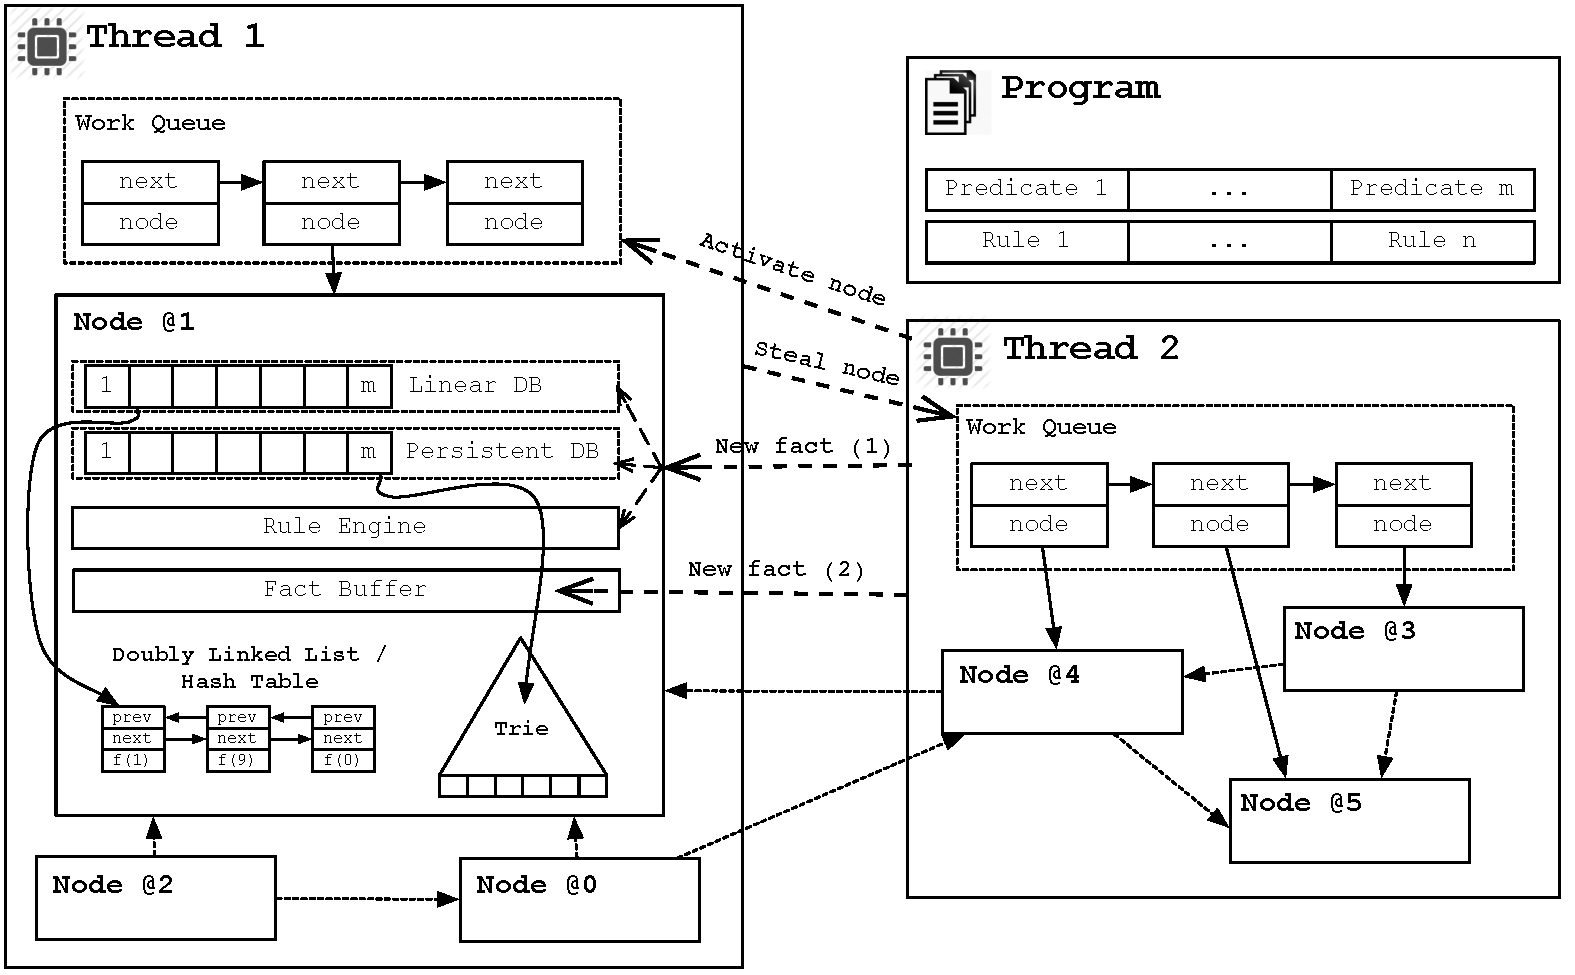
\includegraphics[width=\textwidth]{figures/overview.pdf}
\caption{Layout of the virtual machine}
\label{fig:overview}
\end{figure*}

Figure~\ref{fig:overview} presents the layout of our virtual machine
for a program with six nodes and two running threads. Each thread
space includes the nodes owned by the thread (the dotted arrows
represent the edges between nodes) and a \emph{Work Queue}, a single
linked list containing \emph{active nodes}, i.e., nodes that have new
facts to process. Initially, the \emph{Work Queue} is filled with all
the nodes of the thread in order to derive the
axioms. Figure~\ref{fig:overview} also illustrates the internal
structure layout of a node, which includes: the database of linear
facts (\emph{Linear DB}); the database of persistent facts
(\emph{Persistent DB}); the rule matching structures (\emph{Rule
Engine}); and an auxiliary buffer for storing intermediate facts
coming from other threads (\emph{Fact Buffer}).

Whenever a new fact is derived through rule derivation, we need to
update the data structures for the corresponding node. This is trivial
if the thread that derived the fact also owns the node. If that is not
the case, then we have to synchronize since multiple threads might be
updating the same node's data structures. We added a lock and a
boolean flag to each node to protect the access to its data
structures. When the flag is activated, it means that the node is
currently being executed by the owning thread. For example, in
Fig.~\ref{fig:overview}, if thread 2 derives a fact to
node \texttt{@1} (owned by thread 1), then thread 2 checks the node's
flag and if not activated, will lock node \texttt{@1} and perform the
required updates (\emph{New fact (1)}). If the flag is activated, it
will not touch the main node data structures, but instead will add the
new fact to \emph{Fact Buffer} (\emph{New fact (2)}). The facts stored
in \emph{Fact Buffer} will then be processed whenever the
corresponding node's flag becomes active.

There is another thread interaction that might happen during fact
derivation if the node receiving a new fact is not active. In such
case, the sending thread needs to activate the node by pushing it to
the \emph{Work Queue} of the target thread. For example, consider
again the situation in which thread 2 sends a new fact to
node \texttt{@1}. If node \texttt{@1} is not active, then thread 2
also needs to activate it by pushing it to the \emph{Work Queue} of
thread 1. After this synchronization point, if the target thread is
currently idle, it will become active and with a new node to process.

%%%%%%%%%%%%%%%%%%%%%%%%%%%%%%%%%%%%%%%%%%%%%%%%%%%%%%%%%%%%%%%%%%%%%%

\subsection{Database Data Structures}
\label{sec:database}

We said before that LM rules are constrained by the first argument and
that each node has its own database of linear and persistent
facts. Moreover, since only one thread at a time will be using a
node's database, we do not need to deal with synchronization
issues. Note also that the first argument of each fact is not stored.

The database must be implemented efficiently because during matching
of rules we need to restrict the facts using a given \emph{match
object}, which fixes arguments of the target predicate to instantiated
values. Each node's database is implemented using three kinds of data
structures:

\begin{itemize}
\item \emph{Trie Data Structures} are used exclusively to store 
  persistent facts. Tries are trees where facts are indexed by common
  prefix arguments.
\item \emph{Doubly Linked List Data Structures} are used to store 
  linear facts. We use a double linked list because it is a very
   efficient way to add and remove facts.
\item \emph{Hash Table Data Structures} are used to improve lookup when 
  linked lists are too long and when we need to do search filtered by
  a fixed argument. The virtual machine decides which arguments are
  best to be indexed (see Section~\ref{indexing}) and then uses a hash table
  indexed by the appropriate argument. If we need to go through all
  the facts, we just iterate through all the facts in the table. For
  collisions, we use the above doubly linked list data structure.
\end{itemize}

Figure~\ref{fig:hash_table} shows an example for a hash table data
structure for a \texttt{a(int,int)} predicate with 3 linear facts
indexed by the second argument and stored as a doubly linked list in
bucket \texttt{2}. Each linear fact contains the regular list
pointers, a \texttt{flags} field and the fact arguments. Those are all
stored continuously to improve data locality. One use of
the \texttt{flags} field is to mark that a fact is already being
used. For example, consider the rule:

{\footnotesize
\begin{Verbatim}
a(A,B), a(C,D) -o ...
\end{Verbatim}
}

When we first pick a fact for \texttt{a(A, B)} from the hash
table, we mark it as being used in order to ensure that, when we
retrieve facts for \texttt{a(C, D)}, the first one cannot be used
twice since that would violate linearity.

\begin{figure}[ht]
\centering
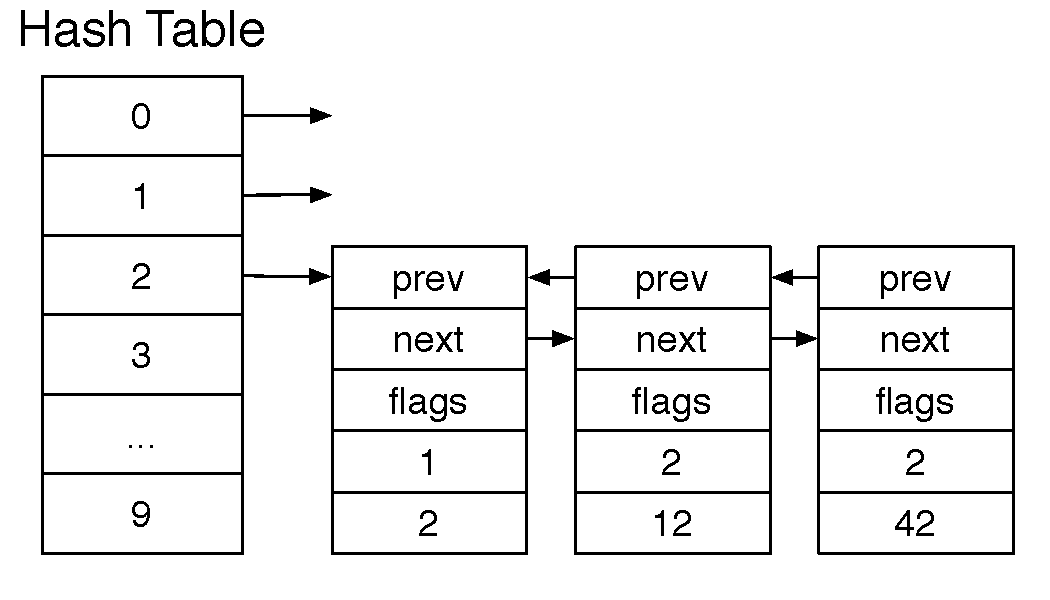
\includegraphics[width=0.4\textwidth]{figures/hash_table.pdf}
\caption{Hash table and doubly linked data structures for 
  a \texttt{a(int,int)} predicate}
\label{fig:hash_table}
\end{figure}

%%%%%%%%%%%%%%%%%%%%%%%%%%%%%%%%%%%%%%%%%%%%%%%%%%%%%%%%%%%%%%%%%%%%%%

\subsection{Rule Engine}
\label{rule_engine}

The rule engine decides which rules may need to be executed while
taking into account rule priorities. Figure~\ref{fig:rule_engine}
shows the rule engine data structures in more detail. There are 4 main
data structures for scheduling rule execution: \texttt{Rule Queue} is
the bitmap representing the rules scheduled to run; \texttt{Active
Bitmap} contains the rules that have enough facts to be
fired; \texttt{Dropped Bitmap} contains the rules that must be dropped
from \texttt{Rule Queue} and \texttt{Active Bitmap} if the rule being
executed succeeds; and \texttt{Predicates Count} counts the number of
facts per predicate. To understand how our engine works, consider the
following set of facts and rules:

{\footnotesize
\begin{Verbatim}
a.
e(0).

a, e(1) -o b.  // rule 1
a -o c.        // rule 2
b -o d.        // rule 3
e(0) -o f.     // rule 4
c -o e(1).     // rule 5
\end{Verbatim}
}

\begin{figure*}[t]
\centering
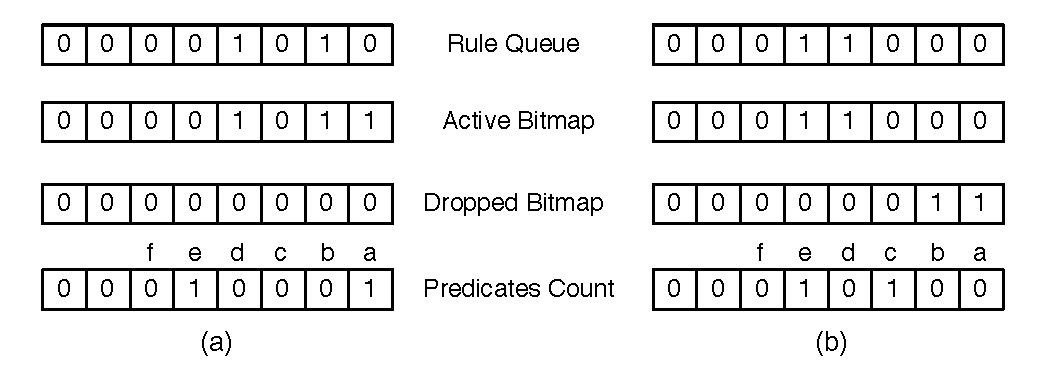
\includegraphics[width=11cm]{figures/rule_queue.pdf}
\caption{Rule engine data structures (a) before and (b) after applying 
  the rule \texttt{a -o c.}}
\label{fig:rule_engine}
\end{figure*}

Since we have facts for predicates \texttt{a/0} and \texttt{e/1},
the \texttt{Active Bitmap} starts with rules 1, 2 and 4 marked as
having enough facts to be fired. The \texttt{Rule Queue} bitmap also
starts with the same three rules. In order to pick rules for
execution, we take the rule corresponding to the least significant bit
from the \texttt{Rule Queue} bitmap, initially the first
rule \texttt{a, e(1) -o b}. However, since we don't have
fact \texttt{e(1)}, this rule fails and we execute the second
rule \texttt{a -o c}. Figure~\ref{fig:rule_engine}(a) shows the rule
engine data structures at that point.

Because the derivation for the second rule succeeds, we will consume
fact \texttt{a} and derive fact \texttt{c}. We thus update
\texttt{Predicates Count} accordingly, mark the first 
and second rules in \texttt{Dropped Bitmap} since such rules are no
longer applicable (\texttt{a} was consumed) and mark the fifth rule
in \texttt{Active Bitmap} since \texttt{c} was derived. Finally, to
update the \texttt{Rule Queue}, we remove the bits marked
in \texttt{Dropped Bitmap} and add the active rules marked
in \texttt{Active Bitmap} that use the newly derived predicates, rule
5 in this case. In the continuation, the engine will schedule the
fourth and fifth rules to run. Figure~\ref{fig:rule_engine}(b) shows
the rule engine data structures at that point.

Note that every node in the program has the same set of data
structures presented in Fig.~\ref{fig:rule_engine}. We use 32 bits
integers to implement the 3 bitmaps and an array of 16 bits integers to
count facts.

We do a small optimization to reduce the number of derivations of
persistent facts and, for that, we divide the program rules into two
sets: \emph{persistent rules} and \emph{non persistent rules}.
Persistent rules are rules where only persistent facts are
involved. We compile such rules incrementally, i.e., we attempt to
fire all rules where a persistent fact is used. This is called
the \emph{pipelined semi-naive} evaluation and it originated in the P2
system~\cite{Loo-condie-garofalakis-p2}. This evaluation method avoids
excessing re-derivations of the same fact. The order of derivation
does not matter for those rules, since only persistent facts are used.

%%%%%%%%%%%%%%%%%%%%%%%%%%%%%%%%%%%%%%%%%%%%%%%%%%%%%%%%%%%%%%%%%%%%%%

\subsection{Rule Execution}

A byte-code file contains meta-data about the program's predicates,
initial nodes, partitioning information, and code for each rule. Each
VM thread has 32 registers that are used during rule
execution. Registers can store facts, integers, floats, node addresses
and pointers to runtime data structures (lists and structures). When
registers store facts, we can reference fields in the fact through the
register.

Consider the example in Fig.~\ref{fig:byte_code} that shows the LM
byte-code for the rule \texttt{!a(X,Y), b(X,Z), c(X,Y) -o
d(Y)}. Consider also a database with the
facts \texttt{!a(1,2)}, \texttt{!a(2,3)}, \texttt{b(1,3)},
\texttt{b(5,3)}, \texttt{c(1,2)}, \texttt{c(1,3)}, \texttt{c(5,3)}. Rule
execution for this rule and facts proceeds in a series of recursive
loops, as follows. The first loop retrieves an iterator for the
persistent facts of \texttt{!a/2} and moves the first valid
fact, \texttt{!a(1,2)}, to register 0. The inner loop retrieves linear
facts that match \texttt{b(1,Z)} (from the
\emph{join constraint}) and moves \texttt{b(1,3)} to register 1. The 
final loop moves \texttt{c(1,2)} to register 2 and the body of the
rule is successfully matched. Next, we derive \texttt{d(2)},
where \texttt{2} comes from register 0.

\begin{figure}[ht]
{\footnotesize
\begin{Verbatim}
PERSISTENT ITERATE a MATCHING TO reg 0
   LINEAR ITERATE b MATCHING TO reg 1
      (match).0=0.0                  // match argument X
      LINEAR ITERATE c MATCHING TO reg 2
         (match).0=0.0               // match argument X
         (match).1=0.1               // match argument Y
         ALLOC d TO reg 3
         MVFIELDFIELD 0.1 TO 3.0       // get argument Y
         ADDLINEAR reg 3                  // derive d(Y)
         REMOVE reg 2
         REMOVE reg 1
         TRY NEXT
      NEXT
   NEXT
RETURN
\end{Verbatim}
}
\caption{LM byte-code for rule \texttt{!a(X,Y), b(X,Z), c(X,Y) -o d(Y)}}
\label{fig:byte_code}
\end{figure}

In case of failure, we jump to the previous loop in order to try the
next candidate fact. In case of rule success, the head is derived and
we should backtrack to the inner most \emph{valid loop}, i.e., the
older loop that uses linear facts or, if there are no linear facts
involved, to the previous loop. We need to jump to a valid loop
because we may have loops with linear facts that are now invalid. In
our example, we would jump to the loop of \texttt{b(X,Z)} and
not \texttt{c(X,Y)}, since \texttt{b(1,3)} was consumed.

As an optimization, the compiler re-orders the fact expressions used
in the body in order to make execution more efficient. For example, it
forces the join constraints in rules to appear first so that matching
will fail sooner rather than later. It also does the same for
constraints. Note also that for every loop, the compiler adds
the \emph{match object}, which contains information about which
arguments need to match, so that runtime matching be efficient.

Our compiler also detects cases where we re-derive a linear fact with
new arguments. For example, as shown in Fig.~\ref{code:update}, the LM
byte-code for rule \texttt{a(N) -o a(N+1)} will compile to code that
reuses/updates the old \texttt{a(N)} fact when deriving the
new \texttt{a(N+1)} fact.

\begin{figure}[ht]
{\footnotesize
\begin{Verbatim}
LINEAR ITERATE a MATCHING TO reg 0
   MVFIELDREG 0.0 TO reg 1           // initial argument
   MVINTREG INT 1 TO reg 2
   reg 1 INT PLUS reg 2 TO reg 3
   MVREGFIELD reg 3 TO 0.0      // reuse/update argument
   UPDATE reg 0
   TRY NEXT
RETURN
\end{Verbatim}
}
\caption{\small{LM byte-code for rule \texttt{a(N) -o a(N+1)}}}
\label{code:update}
\end{figure}

%%%%%%%%%%%%%%%%%%%%%%%%%%%%%%%%%%%%%%%%%%%%%%%%%%%%%%%%%%%%%%%%%%%%%%

\subsection{Indexing}
\label{indexing}

To improve fact lookup, the VM employs a fully dynamic mechanism to
decide which argument may be optimal to index.  The algorithm is
performed in the beginning of the execution and empirically tries to
assess the argument of each predicate that more equally spreads the
database across the values of the argument.  A single thread performs
the algorithm for all predicates.

The indexing algorithm is performed in three main steps. First, it
gathers statistics of lookup data by keeping a counter for each
predicate's argument.  Every time a fact search is performed where
arguments are fixed to a value, the counter of such arguments is
incremented. This phase is performed during rule execution for a small
fraction of the nodes in the program.

The second step of the algorithm then decides the candidate arguments
of each predicate.  If a predicate was not searched with any fixed
arguments, then it will be not indexed.  If only one argument was
fixed, then such argument is set as the indexing argument. Otherwise,
the top 2 arguments are selected for the third phase,
where \emph{entropy statistics} are collected dynamically.

During the third phase, each candidate argument has an entropy score.
Before a node is executed, the facts of the target predicate
are used in the following formula applied for the two arguments:

{\tiny
\[
Entropy(A, F) = - \sum_{v \in values(F, A)} \frac{count(F, A = v)}{total(F)} \log_2 \frac{count(F, A = v)}{total(F)}
\]
}

\noindent
where $A$ is the target argument, $F$ is the set of linear facts
for the target predicate, $values(F, A)$ is set of values of the
argument $A$, $count(F, A = v)$ counts the number of linear facts
where argument $A$ is equal to $v$ and $total(F)$ counts the number of
linear facts in $F$.  The entropy value is a good metric because it
tells us how much information is needed to describe an argument.  If
more information is needed, then that must be the best argument to
index.

For one of the arguments to score, $Entropy(A, F)$ multiplied by the
number of times it has been used for lookup must be larger than the
other argument. The argument with the best score is selected and then
a global variable called \texttt{indexing\_epoch} is updated.  In
order to convert the node's linked lists into hash tables, each node
also has a local variable called \texttt{indexing\_epoch} that is
compared to the global variable in order to rebuild the node database
according to the new indexing information.

Our VM also dynamically resizes the hash table if necessary. When the
hash table becomes too dense, it is resized to the double. When it
becomes too sparse, it is reduced in half or simply transformed back
into a doubly linked list. This is done once in a while, before a node
executes.

We have seen very good results with this scheme. For example, for the
all-pairs shortest paths program, we obtained a 2 to 5-fold
improvement in sequential execution time.  The overhead of dynamic
indexing is negligible since programs run almost as fast as if the
indices have been added from the start.

%%%%%%%%%%%%%%%%%%%%%%%%%%%%%%%%%%%%%%%%%%%%%%%%%%%%%%%%%%%%%%%%%%%%%%

\subsection{Runtime Data Structures}

LM also supports recursive types such as lists and pairs. These
complex data structures are stored in the heap of the VM and are
managed through reference counting. For instance, each list is
a \emph{cons cell} with 3 fields: \texttt{tail}, the pointer to the
next element of the list; \texttt{head}, the element stored by this
element of the list; and \texttt{refs} that counts the number of
pointers to this list element in the VM. The list is deleted from the
heap whenever \texttt{refs} is decremented to zero.

We avoid garbage collection schemes since objects are created and discarded
in very specific points of the virtual machine and our objects cannot contain circular references.
A reference counting mechanism is thus more appropriate than a parallel garbage collector which
would entail pausing the execution of the program to garbage collect all the unused objects.
